\chapter{A LUZ COMO MATERIAL E O CUBO PRETO}

Segundo \citeonline[p. 1]{azevedo} a problemática da luz atravessa a história da arte, de finais do século XIX e durante o século XX. A função da luz não é mais somente de iluminar, de tornar visível uma obra ou um objeto, ou o mero reflexo dos seus efeitos suspensos no espaço. A luz passa a ser tratada como objeto ou material. Na perspectiva da arte contemporânea, se vê que, em muitas obras, a luz passa à matéria. \citeonline[p. 50]{brandi} destaca que "alguns artistas e movimentos estéticos estão fortemente relacionados com a linguagem da luz, mesmo quando não a utilizam como objeto central da obra". 

De acordo com \citeonline[p. 18]{vega} os artistas, em diferentes épocas, se viram inspirados e cativados pela luz, tanto a natural quanto a artificial, e tentaram capturar seu mistério e sua natureza mágica em suas criações. Alguns em particular, como Caravaggio, Vermeer e Monet, buscaram retratar, quase como uma obsessão, a luz e seus efeitos no mundo ao seu redor e, mais recentemente, os artistas contemporâneos vem se utilizando da luz como matéria-prima, realizando manipulações em três dimensões para projetar suas dimensões infinitas. \citeonline[p. 23]{vega} afirma também que, atualmente, muitos artistas exploram as possibilidades da luz artificial, trabalhando com mescla de materiais e diversos tipos de fontes de luz. 

Outro artista cuja obra é relevante no contexto deste trabalho e que, além da luz, explora a perspectiva da arte computacional, é o japonês Takahito Matsuo que, segundo \citeonline[p. 5]{soares}, cria mundos interativos de fantasia e de luz que fazem parte de uma estética enigmática, misturando som e luz perante os movimentos do observador. Seu trabalho destaca as diferentes gradações de luz e sombra que contrastando mostram um mundo de fantasia e imaginação. Em \textit{Fantasias Aquáticas Iluminadas} (figura \ref{fig:takahito_matsuo}), a exploração através de luz, projeções, arquitetura e interações humanas é fortemente encorajada. À medida que os visitantes se aproximam das paredes, se movimentam e se afastam, o número e a frequência das medusas aumentam e diminuem. As formas orgânicas e a brilhante paleta de azúis criam um mundo subaquático surreal, onde movimentos lúdicos e interações com o espaço arquitetônico resultam em uma comunicação não dita entre artista e participante. 

\begin{figure}[H]
    \centering
    \caption{Fantasias Aquáticas Iluminadas, Takahito Matsuo, 2009}
	\vspace*{0,2cm}
    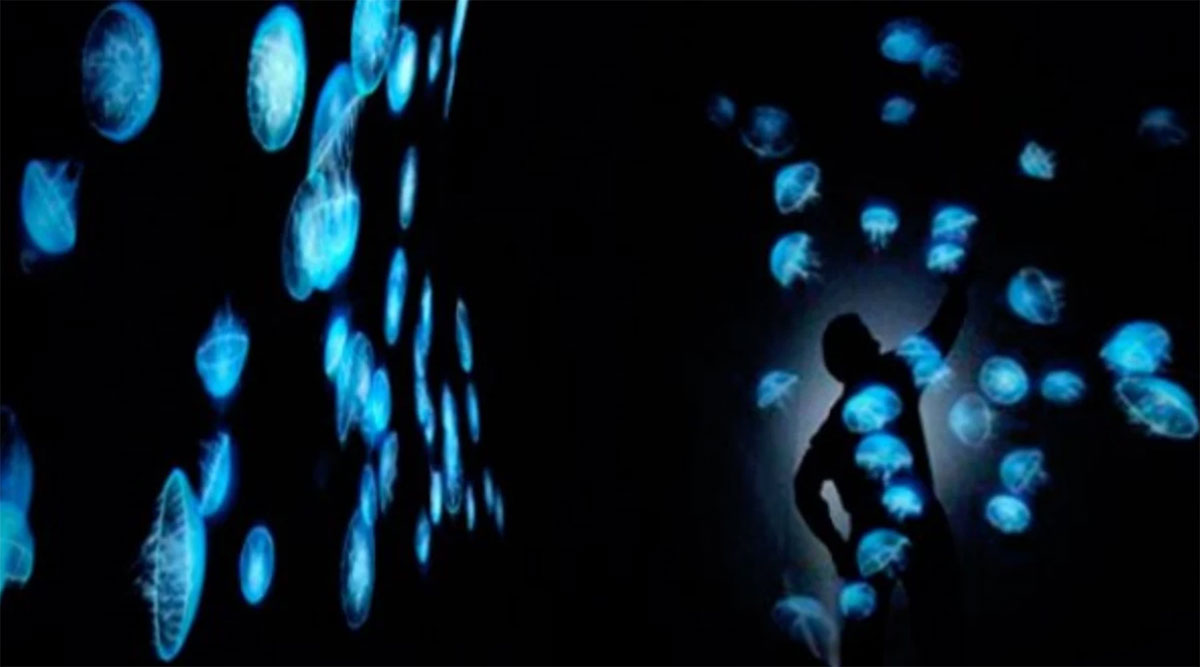
\includegraphics[width=0.8\textwidth]{./04-figuras/takahito_matsuo}
    \label{fig:takahito_matsuo}
\end{figure}
\vspace*{-0,9cm}
{\raggedright \fonte{\citeonline{soares}}}\\

Já o trabalho de Jim Campbell chama à atenção pela antítese presente em suas obras. Em um vídeo produzido pela \citeonline{kqed}, o artista constata que em um mundo de alta definição e telas cada vez mais finas usa tecnologia para produzir o contrário: imagens borradas e em baixa resolução em painéis tridimensionais. Não há projeção. Essas vídeo-esculturas (figura \ref{fig:jim_campbell}) são compostas por grades de LEDs que atuam como uma televisão de pixels desconstruída. De perto, as luzes piscam de maneira desordenada, sendo apenas uma constelação de pontos brilhantes sem muito significado. A peça só começa a se revelar quando o espectador se afasta, tornando-se primeiro uma uma onda sincronizada de luzes em movimento depois se transformando em imagens de crianças brincando ou homens e mulheres caminhando. 

\begin{figure}[H]
    \centering
    \caption{Light Topography Wave, Jim Campbell, 2014}
	\vspace*{0,2cm}
    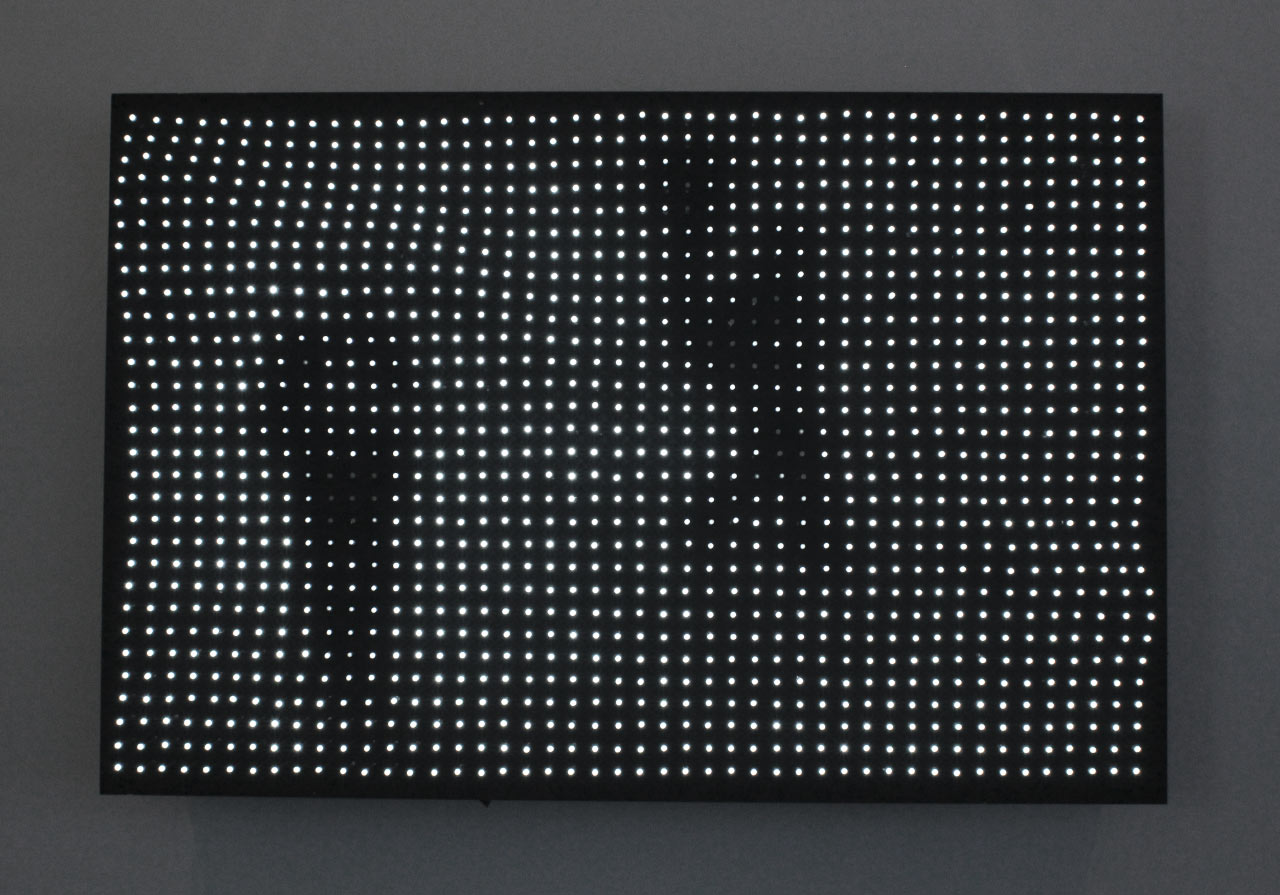
\includegraphics[width=0.8\textwidth]{./04-figuras/jim_campbell}
    \label{fig:jim_campbell}
\end{figure}
\vspace*{-0,9cm}
{\raggedright \fonte{Disponível em: <https://design-milk.com/pixelated-led-art-jim-campbell/>. Acesso em: 22 mar. 2018}}\\

Do ponto de vista da propagação da luz, o cubo branco tende a não ser o cenário ideal para exibição deste tipo de obra. Além disso, \citeonline[p. 40]{soares}, afirma que "a maioria dos autores que trabalham com arte e tecnologia procuram o espaço do cubo preto como espaço expositivo. Neste espaço o que interessa é um novo ver, um espanto com a imagem". Diz ainda que o nome cubo preto para este tipo de exposição surge em contraposição ao cubo branco, criado por Brian O'Doherty, num ensaio publicado pela revista Artforum em 1976, fazendo alusão ao espaço das galerias de arte, com paredes brancas, sem janelas isolando o espetador num meio aparentemente atemporal. A ideia do cubo preto surge como ambiente ideal para propagação da luz e é também uma forma de imersão no interior da mente do artista.


\section{A LUZ NA HISTÓRIA DA ARTE}

De acordo com  \citeonline[p.73]{henno} desde os primórdios da humanidade, quando o homem descobria o fogo, a luz sempre desencadeou fascínio. Esse deslumbramento se manifesta de maneiras distintas ao longo da história da arte. \citeonline{muga} afirma que "a experiência da luz atravessou três paradigmas ao longo da história: o paradigma da luz atributo - a luz venerada; o paradigma da luz efeito - a luz domesticada; e o paradigma da luz causa - a luz instrumentalizada".

Referindo-se à luz venerada, \citeonline{muga}, observa que a luz é percebida essencialmente como um atributo dos objetos, uma propriedade que lhes é inerente e não como um resultado da iluminação. De acordo com \apudonline{arnheim}{muga} até o Renascimento a luz era usada basicamente como um meio de modelar o volume e não enquanto efeito da iluminação. Nesse contexto, o mundo é claro, os objetos são por si só luminosos e as sombras são aplicadas para sugerir rotundidade. Destaca também que na arte religiosa, os fundos dourados, as auréolas, as línguas de fogo, aparecem como atributos brilhantes, representações simbólicas da luz divina e não como reflexo de uma fonte luminosa. Podemos ver um exemplo destes atributos na obra \textit{A lamentação} (figura \ref{fig:giotto_lamentacao}) de Giotto de Bondone.

\begin{figure}[H]
    \centering
    \caption{\textit{A lamentação} (1305), Giotto de Bondone}
	\vspace*{0,2cm}
    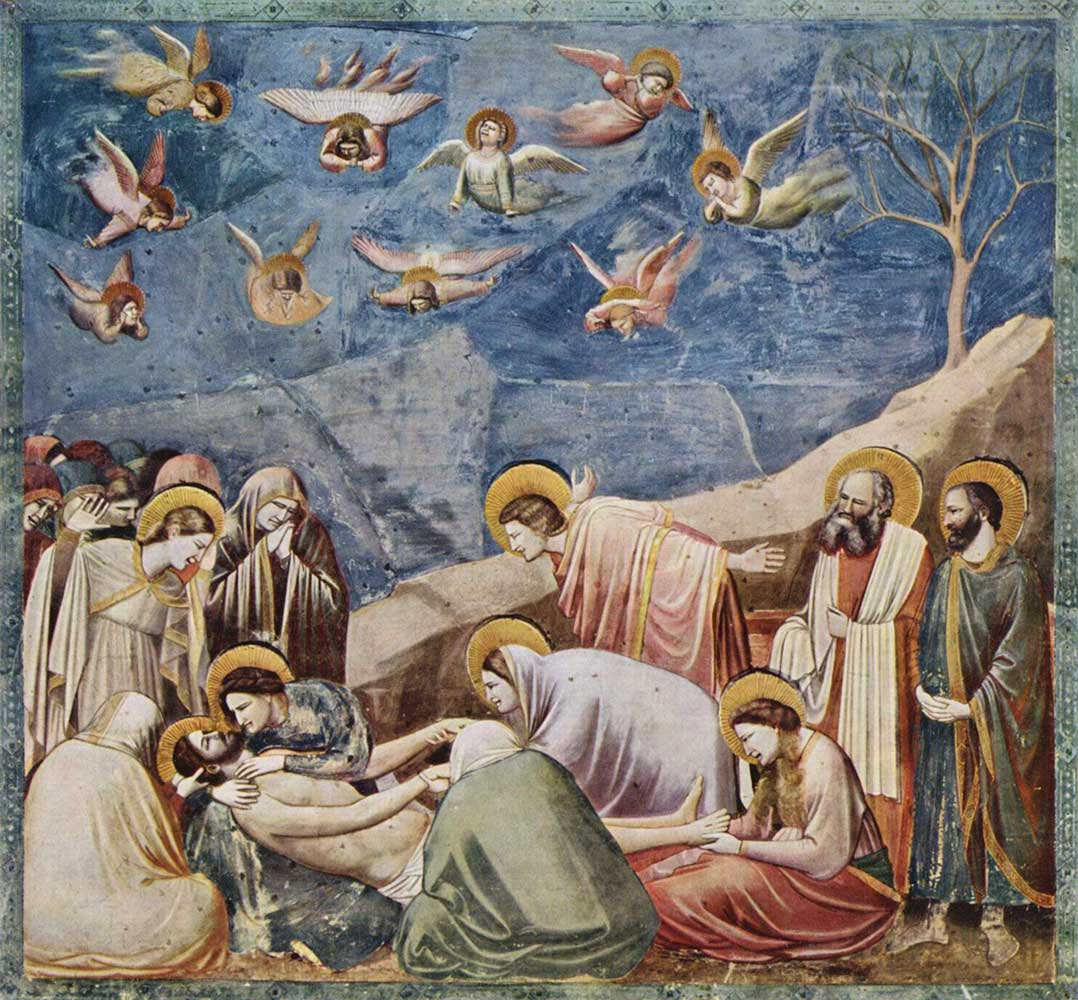
\includegraphics[width=0.8\textwidth]{./04-figuras/giotto_lamentacao}
    \label{fig:giotto_lamentacao}
\end{figure}
\vspace*{-0,9cm}
{\raggedright \fonte{\citeonline{muga}}}\\

\citeonline{muga} relata que é a partir do Renascimento que o paradigma da luz atributo da lugar ao da luz efeito. Além disso, conclui que foi mergulhando na camara obscura que vários pintores do barroco e do renascimento perseguiram uma representação realista da natureza. E que, graças à ela Leonardo da Vinci desenvolveu o método claro-escuro e o \textit{sfumato}, reforçando a tridimensionalidade e a profundidade da representação, evidenciando, assim, o efeito da luz incidente e das partículas atmosféricas na difusão da luz. Esse estudo,  como podemos ver na figura \ref{fig:da_vinci_virgem_rochedos}, \textit{A virgem dos rochedos} de Leonardo da Vinci, é desenvolvido no seio da escuridão que, como afirma \citeonline{muga}, antes atributo do mal, torna-se aliada para se chegar à luz.

\begin{figure}[H]
    \centering
    \caption{\textit{A virgem dos rochedos} (1495-1508), Leonardo da Vinci}
	\vspace*{0,2cm}
    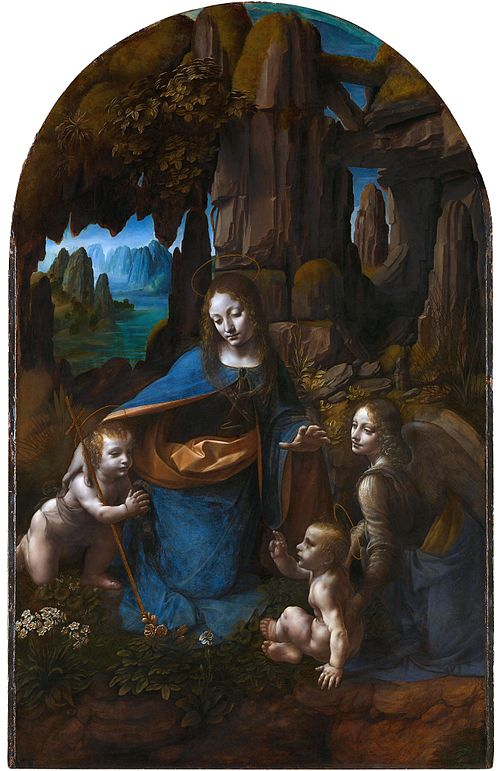
\includegraphics[width=0.5\textwidth]{./04-figuras/da_vinci_virgem_rochedos}
    \label{fig:da_vinci_virgem_rochedos}
\end{figure}
\vspace*{-0,9cm}
{\raggedright \fonte{\citeonline{muga}}}\\


Com o advento da fotografia os pintores precisaram se reinventar. Para \citeonline[p. 77]{henno} "o progresso tecnológico atrelado a fotografia exigiu que os artistas deslocassem o hábito descritivo da mimesis para um desenvolvimento interno de sua criatividade". Voltando a \citeonline{muga}, a fotografia influenciou os impressionistas a saírem do ateliers e procurarem no interior do globo ocular a percepção de uma natureza que, a cada mutação de luz, mudava de aspecto e de verdade. Segundo \apudonline{gombrich}{muga} Édouard Manet e seus seguidores descobriram que "ao olharmos a natureza ao ar livre e à plena luz do dia, as formas redondas parecem planas, e não vemos os objetos cada um com a sua cor própria, mas uma mistura brilhante de matizes que se combinam nos nossos olhos".


De acordo com \citeonline[p. 78]{henno} foi apoiado no preceito de que a cor se mistura no olho e não na paleta que Seurat aplicava pontos de cor na tela, em locais estratégicos, a fim de que a mistura desses pontos, a partir de uma distância apropriada, fossem vistos como uma única cor pelo observador. Na figura \ref{fig:seurat_la_parede_detalhe} podemos ver o detalhe da obra \textit{La Parede} (figura \ref{fig:seurat_la_parede}) deste artista.

\begin{figure}[H]
    \centering
    \caption{\textit{La Parade} (1887-88), Georges Seurat}
	\vspace*{0,2cm}
    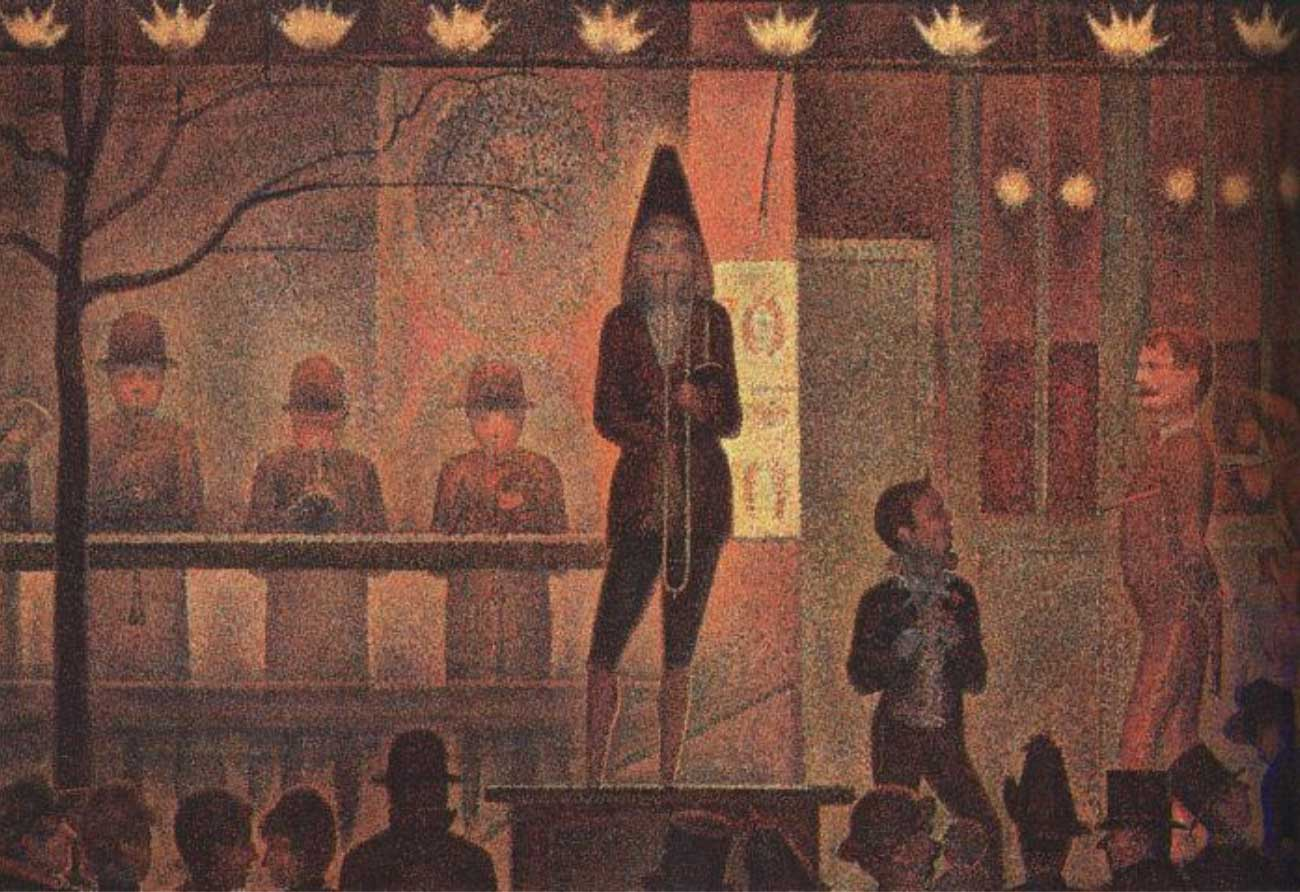
\includegraphics[width=0.8\textwidth]{./04-figuras/seurat_la_parede}
    \label{fig:seurat_la_parede}
\end{figure}
\vspace*{-0,9cm}
{\raggedright \fonte{\citeonline[p.79]{henno}}}\\
   
\begin{figure}[H]
    \centering
    \caption{\textit{La Parade} (1887-88) - detalhe ampliado, Georges Seurat}
	\vspace*{0,2cm}
    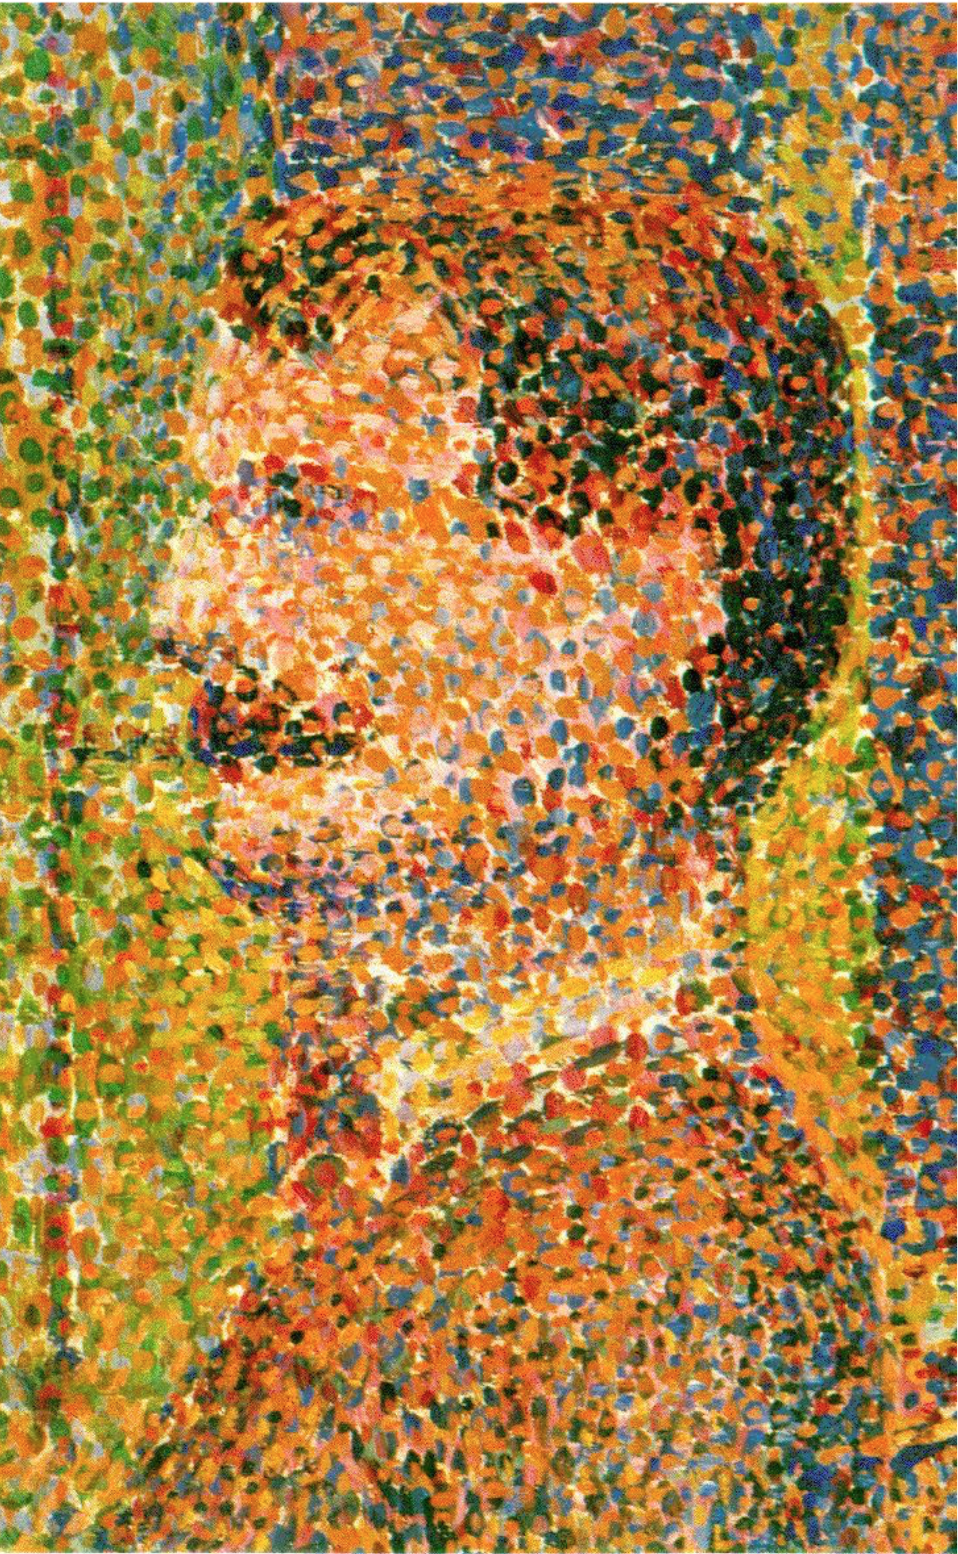
\includegraphics[width=0.5\textwidth]{./04-figuras/seurat_la_parede_detalhe}
    \label{fig:seurat_la_parede_detalhe}
\end{figure}
\vspace*{-0,9cm}
{\raggedright \fonte{\citeonline[p.79]{henno}}}\\

Por fim, como afirma \citeonline{muga}, depois de ocupar o lugar de atributo brilhante e de efeito de iluminação, ao longo so século XX, a luz se torna um material, um meio. James Turrell, por exemplo, foi pioneiro de uma nova preocupação com os fenômenos do espaço e da luz. Em seus primeiros trabalhos investigou os efeitos da luz artificial. Ele também desenvolveu várias instalações que aumentaram a relação entre a luz e a estrutura arquitetônica. Em conversa com \citeonline[p. 114]{adcock}, ele relata que uma das dificuldades de usar a luz é que ainda não é tradição utilizá-la em nossa cultura. Por outro lado, não é mais incomum usá-la do que usar pedra, argila, aço ou tinta. O artista declara seu interesse em trabalhar a luz como material, mas não luz em vidro, fibra de vidro ou acrílico, e sim no próprio espaço e nas qualidades do espaço, fazendo luz sem a forma física tradicional. Ele nos traz também que há uma rica tradição na pintura do trabalho sobre a luz, mas que isso de fato não é luz - é o registro da visão. Na figura \ref{fig:james_turrell} podemos ver sua obra entitulada \textit{The light inside} que transforma as paredes de um túnel em vasos para a condução da luz e nos dá uma ideia da dimensão na qual o artista trabalha este material. 

\begin{figure}[H]
    \centering
    \caption{\textit{The light inside} (1999), James Turrell}
	\vspace*{0,2cm}
    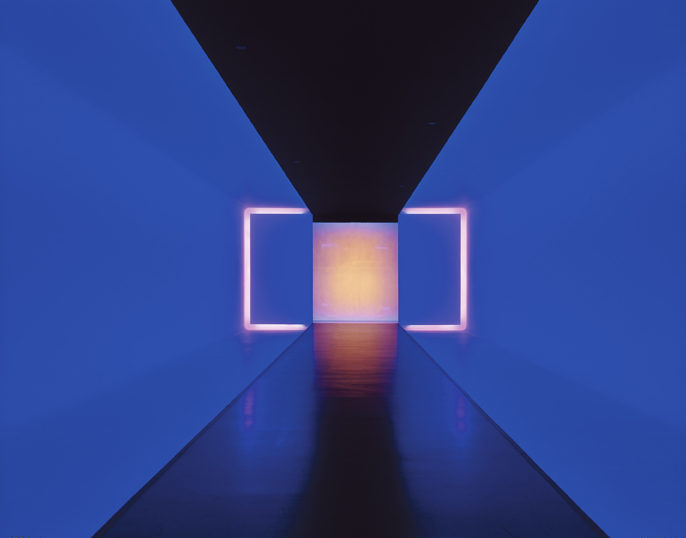
\includegraphics[width=0.8\textwidth]{./04-figuras/james_turrell}
    \label{fig:james_turrell}
\end{figure}
\vspace*{-0,9cm}
{\raggedright \fonte{Disponível em: <http://jamesturrell.com/work/thelightinside/>. Acesso em: 18 jun. 2018}}\\






